\documentclass[11pt,a4paper]{article}

\usepackage[margin=1in]{geometry}
\usepackage{titlesec}
\usepackage{enumitem}
\usepackage{hyperref}
\usepackage{parskip}
\usepackage{graphicx}
\usepackage{float}
\usepackage{booktabs}
\usepackage{amsmath}

\hypersetup{colorlinks=true, linkcolor=blue, urlcolor=blue}

\titleformat{\section}{\large\bfseries}{\thesection}{0.5em}{}
\titleformat{\subsection}{\normalsize\bfseries}{\thesubsection}{0.5em}{}
\setlist{leftmargin=1.4em, topsep=2pt, itemsep=2pt}

\title{\vspace{-1.5cm}\textbf{PKCERT AI \& Software Development Internship \\ Task 18: Intro to PyTorch}}
\author{Abdullah Amir}
\date{AI and Software Development \\ 28 July 2026}

\begin{document}

\maketitle
\vspace{-0.8cm}

This report covers the theory and the results. The full code and outputs live in the
notebook \texttt{intro\_to\_pytorch.ipynb}. \textbf{PyTorch 2.13.0 (CPU build)} is used
throughout. Task 17 built a perceptron, activation functions, and a 2-layer MLP from
scratch in NumPy, with backpropagation verified against finite differences. This task
rebuilds the same architecture on the same dataset in PyTorch, using its autograd engine
and \texttt{nn.Module} API, and maps every concept back to that manual derivation.

% ----------------------------------------------------------------
\section*{Part A: Tensors \& Basic Operations}

\textbf{Four ways to create a tensor}, each suited to a different situation:
\texttt{torch.tensor(list)} for concrete hand-written values; \texttt{torch.zeros}/
\texttt{ones} for placeholders and accumulators of known shape; \texttt{torch.arange}
for index ranges and schedules; \texttt{torch.rand} for weight initialisation and
stochastic sampling; \texttt{torch.from\_numpy} for data that already lives in NumPy and
needs to enter PyTorch without copying.

\textbf{Indexing, slicing, reshaping.} Standard NumPy-style indexing and slicing work
directly on tensors. \texttt{view()} always shares the underlying memory (and requires
the tensor to already be contiguous); \texttt{reshape()} behaves the same way when
possible but silently falls back to copying when the current memory layout does not
support the requested shape -- the safer general-purpose choice, since it never raises
where \texttt{view()} would. \textbf{Broadcasting} follows NumPy's rules exactly: a
$(4,1)$ tensor plus a $(1,3)$ tensor broadcasts to $(4,3)$ with no data copied;
genuinely incompatible shapes, e.g. $(4,2)$ and $(3,2)$, correctly raise a
\texttt{RuntimeError}.

\textbf{Matrix multiplication, NumPy vs PyTorch, timed.} A $1200\times1200$ matmul,
mean of 5 runs: NumPy 32.50ms, PyTorch 45.08ms -- NumPy was 1.39x faster on this CPU.
Both libraries ultimately call into an optimised BLAS library for float64 CPU matmul, so
this gap reflects which BLAS backend each happened to link against on this particular
machine, not an inherent advantage of either library's Python layer.

\textbf{\texttt{torch.Tensor} vs \texttt{numpy.ndarray}.} Demonstrated, not just
described: \texttt{torch.from\_numpy()} and \texttt{.numpy()} both construct a view over
the \emph{same} memory buffer -- mutating a tensor created with \texttt{from\_numpy()}
was confirmed to mutate the original NumPy array, and vice versa via \texttt{.numpy()}.
\texttt{torch.tensor(existing\_array)}, in contrast, always copies: mutating the
resulting tensor left the original array untouched. Underneath the API, a
\texttt{torch.Tensor} and an \texttt{ndarray} are the same kind of object -- a
contiguous memory buffer plus shape/stride/dtype metadata -- which is exactly why the
sharing conversions are free and the copying ones are not.

% ----------------------------------------------------------------
\section*{Part B: Autograd}

\textbf{Computational graph.} A record of every differentiable operation applied to a
tensor, linking each output back to the inputs and operation that produced it -- what
\texttt{.backward()} walks in reverse to apply the chain rule automatically. PyTorch
builds this \textbf{dynamically} (``define-by-run''): no graph exists before any code
runs; each operation appends a node \emph{as it actually executes}, which is why
ordinary Python control flow works transparently inside a PyTorch model.

\textbf{A scalar check.} $y = x^2 + 3x + 1$ at $x=3.0$: autograd gives
$dy/dx = 9.0$; by hand, $2x+3 = 9.0$. Match confirmed with \texttt{torch.isclose}.

\textbf{Gradient accumulation.} Calling \texttt{.backward()} three times on
$(w-5)^2$ without resetting \texttt{w.grad} between calls accumulated $-6, -12, -18$ --
each call \emph{adds} to the existing gradient rather than replacing it. This is why
every training loop calls \texttt{optimizer.zero\_grad()} before each new
\texttt{loss.backward()}: without it, every update silently includes every previous
step's leftover gradient (the deliberate exception is genuine gradient accumulation
across mini-batches to simulate a larger batch, where the accumulation is the point).

\textbf{\texttt{torch.no\_grad()} and \texttt{.detach()}, proven rather than asserted.}
Attempting \texttt{weight -= lr * weight.grad} on a leaf tensor with
\texttt{requires\_grad=True}, outside \texttt{no\_grad()}, was run and actually raised:
\texttt{"a leaf Variable that requires grad is being used in an in-place operation"}.
Wrapping the identical line in \texttt{with torch.no\_grad():} succeeded. \texttt{no\_grad()}
is the right tool for a whole block of computation (an evaluation pass, a manual
parameter update); \texttt{.detach()} is for pulling one specific tensor out of the
graph mid-computation (e.g. logging a loss value) without carrying its upstream graph.

\subsection*{Autograd vs Task 17's manual backpropagation}

The exact weights Task 17 trained and saved were loaded, and both the manual NumPy
formulas and PyTorch autograd were run on the identical batch of real penguin data.

\begin{table}[H]
\centering
\begin{tabular}{lr}
\toprule
\textbf{Parameter} & \textbf{Max abs.\ difference, autograd vs manual} \\
\midrule
$W_1$ & $\approx 10^{-17}$ \\
$b_1$ & $\approx 10^{-17}$ \\
$W_2$ & $\approx 10^{-17}$ \\
$b_2$ & $\approx 10^{-17}$ \\
\bottomrule
\end{tabular}
\caption{All four match to machine epsilon for float64 -- essentially exact.}
\end{table}

\textbf{Two independent gradient checks now agree.} Task 17 verified its manual
backprop against finite differences ($\sim10^{-10}$ relative error, an
analytical-vs-numerical-approximation comparison). This check compares the same manual
formulas against PyTorch's autograd -- two \emph{exact} analytical methods -- and they
agree to $\sim10^{-17}$, machine epsilon itself. Autograd is not doing something
different or more mysterious than the hand derivation; it is automating the identical
calculus.

% ----------------------------------------------------------------
\section*{Part C: Building \& Training a Simple Neural Network}

Same dataset (Palmer Penguins, 342 birds, 4 features, 3 species) and architecture
($4 \to 8 \to 3$, ReLU hidden) as Task 17. A fresh \texttt{ManualMLP} (NumPy) and
\texttt{MLPClassifier} (scikit-learn) were also trained in this same run, on the same
split, so all three training times are measured on identical hardware rather than
compared across sessions.

\textbf{Loss and optimizer, justified.} \texttt{nn.CrossEntropyLoss} combines
\texttt{log\_softmax} and negative-log-likelihood in one numerically stable call
(log-sum-exp internally, avoiding the separate softmax-then-clip Task 17 needed by
hand) -- the direct PyTorch analogue of the manually derived softmax+cross-entropy
pair. \texttt{SGD} at the same learning rate as Task 17/sklearn (0.1) is used for the
primary, fair three-way comparison; \texttt{Adam} is explored separately as the
hyperparameter experiment.

\begin{figure}[H]
    \centering
    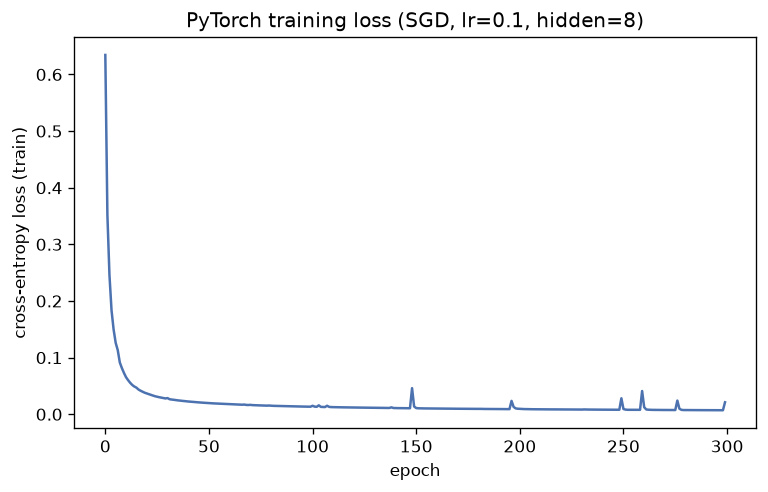
\includegraphics[width=0.62\textwidth]{figures/01_pytorch_loss_curve.png}
    \caption{PyTorch training loss, SGD, 300 epochs.}
\end{figure}

\begin{table}[H]
\centering
\begin{tabular}{lrrrr}
\toprule
\textbf{Implementation} & \textbf{Accuracy} & \textbf{Macro-F1} & \textbf{Fit time} \\
\midrule
ManualMLP (NumPy, Task 17) & 0.9855 & 0.9877 & \textbf{0.110s} \\
sklearn MLPClassifier & \textbf{1.0000} & \textbf{1.0000} & \textbf{0.109s} \\
PyTorch nn.Module (SGD) & \textbf{1.0000} & \textbf{1.0000} & 2.510s \\
\bottomrule
\end{tabular}
\caption{Same 300-epoch, batch-16 schedule, same split, same CPU.}
\end{table}

\begin{figure}[H]
    \centering
    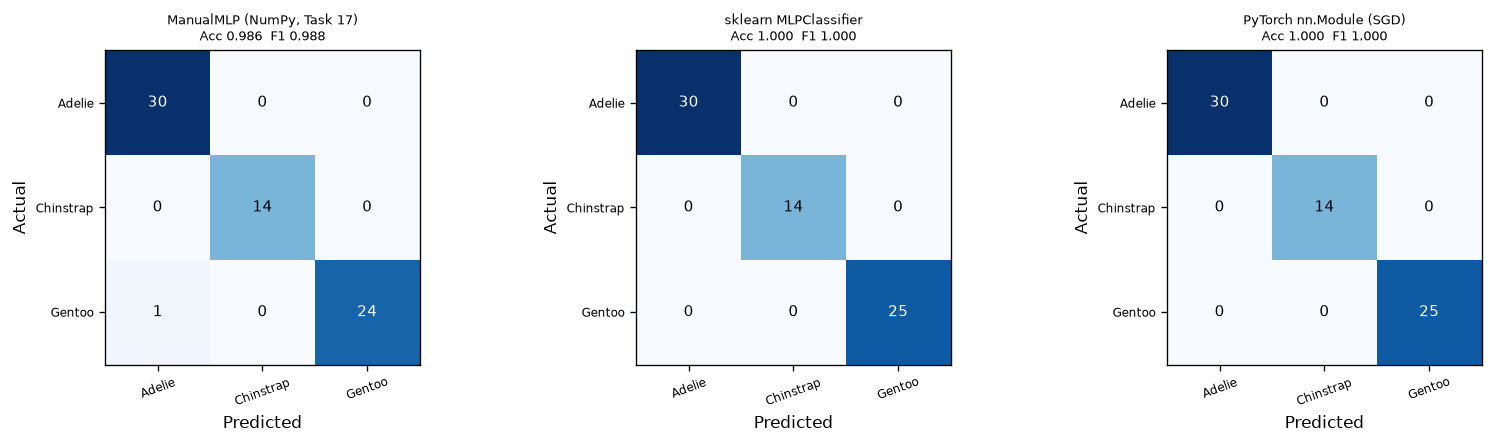
\includegraphics[width=0.95\textwidth]{figures/02_confusion_matrices_3way.png}
    \caption{All three confusion matrices; PyTorch and sklearn are both perfect on this split.}
\end{figure}

\begin{figure}[H]
    \centering
    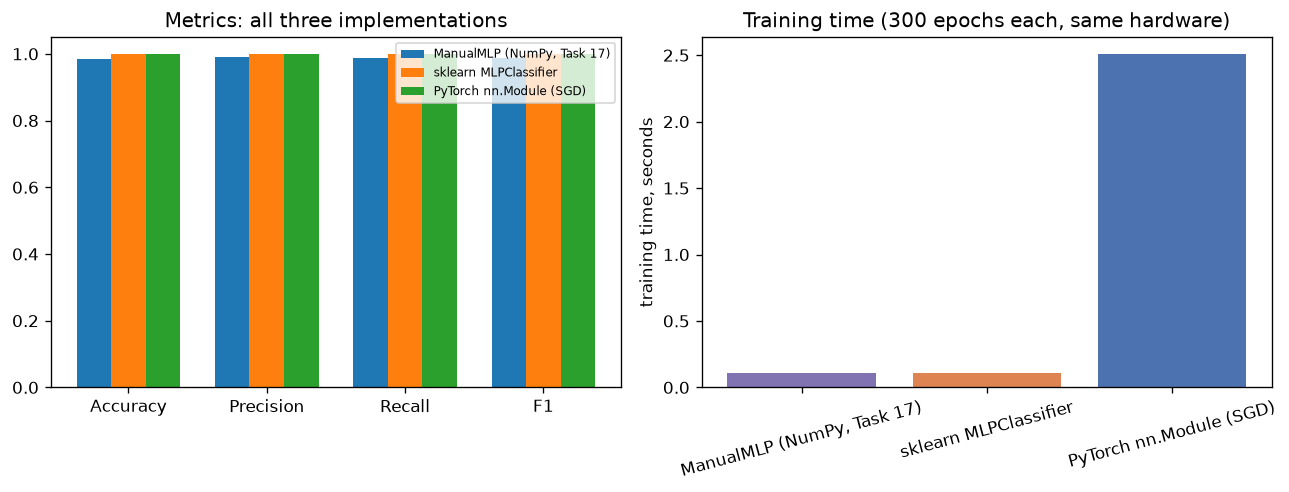
\includegraphics[width=0.95\textwidth]{figures/03_metrics_and_timing.png}
    \caption{Left: metrics across all three. Right: training time -- PyTorch is the outlier.}
\end{figure}

\textbf{PyTorch matched sklearn on accuracy but took roughly 20x longer to train than
either the NumPy or scikit-learn model}, despite all three running the identical
schedule on the same CPU. This is not a criticism of PyTorch -- it is the expected
result of per-operation overhead (building an autograd graph node, Python/C++ dispatch,
gradient bookkeeping for every one of the roughly 5,400 mini-batch steps) dominating
when the actual arithmetic per step is tiny (a $4\times8$ and an $8\times3$ matrix
multiply). Frameworks like PyTorch earn their keep on large models, large batches and
GPU execution, where that per-step overhead becomes negligible next to the computation
itself; on a network this small, the overhead \emph{is} most of the cost.

\subsection*{Hyperparameter experiment: optimizer choice}

\begin{table}[H]
\centering
\begin{tabular}{lrr}
\toprule
\textbf{Optimizer} & \textbf{Final training loss} & \textbf{Test accuracy} \\
\midrule
SGD (lr=0.1) & 0.0212 & \textbf{1.0000} \\
Adam (lr=0.1) & 0.0019 & 0.9855 \\
Adam (lr=0.01) & \textbf{0.0012} & \textbf{1.0000} \\
\bottomrule
\end{tabular}
\end{table}

\begin{figure}[H]
    \centering
    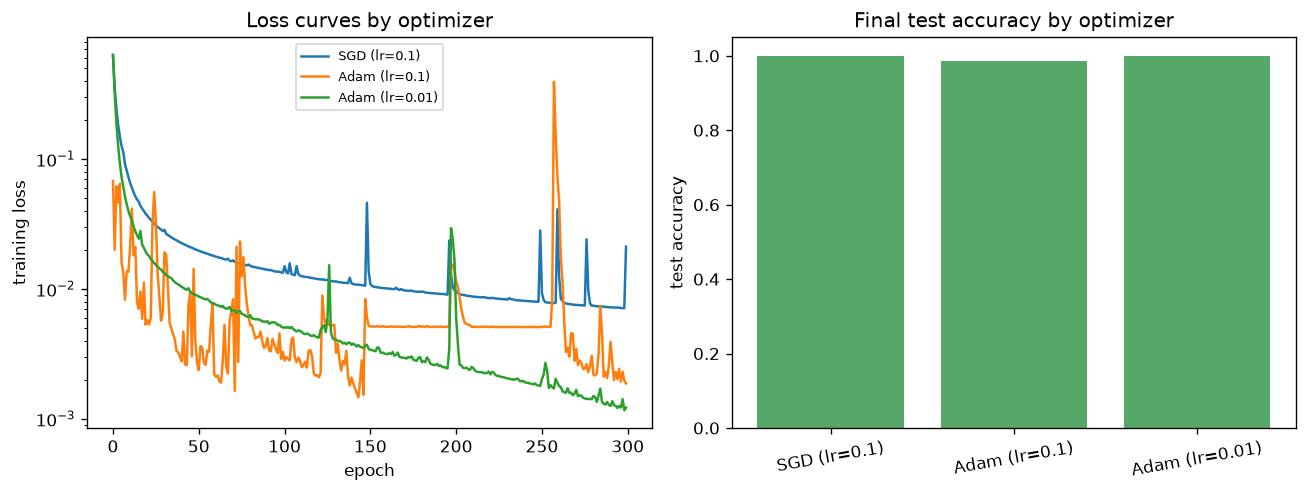
\includegraphics[width=0.95\textwidth]{figures/04_optimizer_experiment.png}
    \caption{Left: loss curves (log scale) by optimizer. Right: final test accuracy.}
\end{figure}

\textbf{Adam at the same learning rate as SGD (0.1) performed \emph{worse}} (98.6\% vs
SGD's 100\%) and its loss curve is visibly noisier -- Adam's adaptive per-parameter
scaling makes its \emph{effective} step size at a given nominal learning rate larger
than plain SGD's, and 0.1 is well outside Adam's typical comfortable range. Dropping to
\texttt{lr=0.01} fixed both symptoms: the smoothest curve of the three and the lowest
final loss, back to 100\% test accuracy. The lesson is specific and checkable, not a
general claim that either optimizer is better: an optimizer swap is not a drop-in
change at a fixed learning rate.

% ----------------------------------------------------------------
\section*{Part D: Analysis \& Documentation}

\textbf{Pipeline summary.} Architecture $4 \to 8 \to 3$ (identical to Task 17):
\texttt{nn.Linear(4,8)} $\to$ ReLU $\to$ \texttt{nn.Linear(8,3)}, raw logits out. Loss:
\texttt{nn.CrossEntropyLoss}. Optimizer for the primary comparison: SGD(lr=0.1),
matching the manual and sklearn baselines exactly; Adam explored separately. 300
epochs, batch size 16 -- identical to Task 17 throughout. The trained model's
\texttt{state\_dict} was saved with \texttt{torch.save} and reloading it with
\texttt{load\_state\_dict} was verified to reproduce identical test predictions.

\textbf{Two concrete differences observed, Task 17 (NumPy) vs this PyTorch
implementation.}
\begin{enumerate}
    \item \emph{Training speed, in the opposite direction most people expect.}
    PyTorch took $\sim$20x longer than the hand-written NumPy version on this tiny
    network, because per-step framework overhead dominates when the actual matrix
    operations are this small. The lesson generalises: a framework's advantage is in
    what it makes \emph{possible} (deeper networks, GPU execution, automatic
    differentiation through arbitrary architectures) and in engineering time, not
    necessarily wall-clock speed on a toy-sized problem.
    \item \emph{Code complexity and the shape of the risk.} The manual implementation
    is roughly 60 lines of NumPy that must be re-derived by hand for any architecture
    change, with the entire correctness burden on getting the calculus and matrix
    orientations right (Task 17 needed an explicit finite-difference check to trust
    it). \texttt{loss.backward()} replaces the entire hand-written \texttt{backward()}
    method, and autograd is correct by construction for any differentiable graph, so
    the risk shifts away from calculus bugs and toward framework-specific mistakes:
    dtype/shape mismatches, forgetting \texttt{zero\_grad()}, or an in-place operation
    on a leaf tensor (the gotcha below).
\end{enumerate}

\textbf{What autograd abstracts away, and why Task 17 still mattered.} Autograd
abstracts away the entire derivation this pipeline depends on: it is never told that
$\partial L/\partial Z_2 = A_2 - Y$, or which axis a bias gradient sums over, or which
matrix to transpose in $dW_1 = X^\top dZ_1$ -- it derives all of that automatically from
the chain rule applied to whatever \texttt{forward()} happens to run. That is exactly
why Task 17 remains valuable even though this task never needs its formulas directly
again: writing and finite-difference-verifying the derivation by hand is what makes it
possible to read a loss curve, a vanishing gradient, or a training instability and know
which piece of the underlying mathematics is responsible, rather than treating
\texttt{loss.backward()} as a button that makes numbers go down. Part B's
$\sim10^{-17}$ agreement between autograd and the Task 17 formulas is the direct proof
that the two compute the same thing.

\textbf{A limitation/gotcha, demonstrated live.} Calling
\texttt{weight -= lr * weight.grad} on a leaf tensor with \texttt{requires\_grad=True},
outside \texttt{torch.no\_grad()}, raises immediately -- PyTorch forbids in-place
updates to such tensors because they would silently corrupt values other operations may
still need during backpropagation. The fix, and the reason \texttt{optimizer.step()}
wraps itself in \texttt{no\_grad()} internally, is to explicitly mark that block of code
as untracked by autograd -- caught and printed directly in Part B rather than only
described in prose.

\textbf{Conclusion.} The thread connecting this task to Task 17 is verification, not
just translation. Every claim here was checked against an independent source: PyTorch's
own tensor semantics were demonstrated with actual shared-memory mutations and an actual
caught \texttt{RuntimeError}, not just described; and, most importantly, PyTorch's
autograd gradients were checked against Task 17's hand-derived formulas on identical
weights and data, agreeing to machine precision. The result is a PyTorch implementation
that reaches the same accuracy as the framework baseline it is meant to reproduce, at a
real and now-quantified cost in training time for a network this small -- evidence that
adopting a production framework is a genuine trade-off, not a strict upgrade, at this
scale.

\vspace{0.4cm}
\noindent The notebook and README are on GitHub: {\small\scalebox{0.72}[1]{\url{https://github.com/AbdullahAmir06/ai-internship-abdullahamir}}}

\end{document}
